\section{The design: where the excitation can be bought, and what it decides}
\label{sec:designsec}
%==========================================================================

\emph{Section~\ref{sec:excitation} says what a trajectory has to do. This section asks
what the accessible trajectories actually do, and what decision the answer supports.}

\subsection{What does not collapse, stays --- and what does, and why}
\label{sec:collapse}

The estimator here is the exact information filter for constant parameters,
\begin{equation}
P_k^{-1} \;=\; P_0^{-1} \;+\; \sum_{i \le k} \frac{q(m_i, \Delta_i)\,q(m_i, \Delta_i)^{\!\top}}{\sigma^2},
\label{eq:infofilter}
\end{equation}
on the augmented coordinates $(\ln\theta, \ln K_m, L_0, \ln k_e)$, none of which carries
dynamics. \textbf{There is no process noise on $\theta$, and that is a construction rather
than a setting.} A random walk on $\theta$ manufactures a finite stationary covariance in a
direction the data may never see, which is precisely the error this note exists to warn
about; with \eqref{eq:infofilter}, what does not collapse stays visibly uncollapsed.

\paragraph{The footing, stated once and used everywhere.} Four choices decide every number
in this section, and earlier drafts of this note did not hold them fixed.
\begin{enumerate}[leftmargin=*, itemsep=2pt]
\item \textbf{$q$ carries the increment}, as \eqref{eq:columns} requires. A design is
\emph{not} fully described by the levels it visits: two samples at the same level under
different $\Delta$ carry different information, and that is the whole of
Section~\ref{sec:therapychannel}.
\item \textbf{$\theta$ and $K_m$ are free.} No prior is placed on either. Stripping the
priors one at a time shows that the $K_m$ prior does no work at all --- the accessible
design gives $0.1474$ with it and $0.1474$ without it, and still $0.1474$ at a prior
twenty times looser --- so nothing here depends on knowing $K_m$, which
Remark~\ref{rem:no_km} forbids.
\item \textbf{$k_e$ carries a log-prior of $0.8$}, a factor of $2.2$, and it is the only
prior that does any work: removing it takes the same design from $0.1474$ to $0.6451$. The
gate needs $k_e$ within a factor of $2.95$, which is the one thing this note asks the
literature for.
\item \textbf{Intake varies day to day at a $10\%$ coefficient of variation, and is
recorded to $5\%$.} By Proposition~\ref{prop:rank} a perfectly steady load is the exactly
singular case, so the variability is not noise to be averaged away.
\end{enumerate}

An extended Kalman filter on the joint state was written first and is not used, for a
reason worth recording. The marker's time constant is
$\bigl((\theta+\Delta) g'(\bar m) + k_e\bigr)^{-1}$, which is $0.81$ hours at the
illustrative values, against a therapeutic increment decaying with a half-life of $3.5$
days: a separation of $104$. The marker is therefore in quasi-steady state at every
sampling instant a clinic could use and \eqref{eq:infofilter} is exact rather than
approximate. The code measures the separation rather than asserting it, and returns one
number a protocol needs: after a dose the marker is within $5\%$ of quasi-steady in $0.91$
hours and tracks to within $5\%$ thereafter, so a sample drawn inside that first hour is
not a steady state and does not belong in a steady-state fit.

\begin{figure}[htbp]
\centering
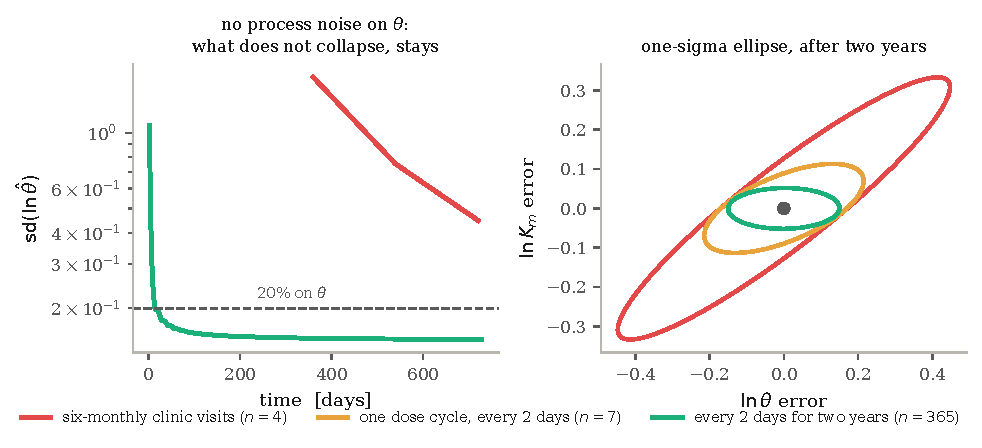
\includegraphics[width=\textwidth]{fig_D2_collapse.pdf}
\caption{Three sampling designs under the biweekly dosing schedule, over two years.
\textbf{Left:} $\operatorname{sd}(\ln\hat\theta)$ as samples arrive. \textbf{Right:} the
one-sigma ellipse in $(\ln\theta, \ln K_m)$ at the end. What separates the designs is how
much of the dose cycle they see, not how many samples they take.}
\label{fig:D2}
\end{figure}

\begin{adjustwidth}{-1.4cm}{-1.4cm}
\begin{table}[htbp]
\centering
\footnotesize
\caption{\label{tab:designs}What each design delivers. Bold is inside the $20\%$ target.
The fourth column is the range of the therapeutic increment the design actually sees, and
it, rather than $n$, is what orders the table. The last column is the same design evaluated
with the increment dropped from the sensitivity while still being used to generate the
levels, which is what earlier drafts of this note reported.}
\begin{tabular}{@{}llllll@{}}
\toprule
\textbf{design} & \textbf{$n$} & \textbf{levels visited} & \textbf{range of $\Delta/\theta$} & \textbf{$\operatorname{sd}(\ln\hat\theta)$} & \textbf{$\operatorname{corr}(\ln\hat\theta, \ln \hat K_m)$} \\
\midrule
six-monthly clinic visits & 4 & $5.76$--$10.34$ & $0.45$ & 0.4570\,\scriptsize$[0.4121, 0.5097]$ & $+0.9278$ \\
one dose cycle, every two days & 7 & $3.28$--$7.79$ & $1.81$ & 0.2162\,\scriptsize$[0.2053, 0.2300]$ & $+0.6137$ \\
\textbf{monthly, across dose cycles} & 25 & $2.81$--$9.47$ & $1.84$ & \textbf{0.1699}\,\scriptsize$[0.1684, 0.1709]$ & $+0.3356$ \\
two-monthly, across dose cycles & 13 & $3.28$--$9.70$ & $1.94$ & \textbf{0.1876}\,\scriptsize$[0.1839, 0.1939]$ & $+0.4711$ \\
every two days for two years & 365 & $2.49$--$10.47$ & $1.95$ & \textbf{0.1500}\,\scriptsize$[0.1498, 0.1501]$ & $+0.0327$ \\
\emph{fortnightly: the dose interval itself} & 53 & $2.39$--$4.53$ & $0.13$ & 4.5845\,\scriptsize$[3.5050, 5.6362]$ & $+0.9990$ \\
\emph{the same $365$ straddling $K_m$} & 365 & $50.00$--$200.00$ & $1.95$ & \textbf{0.0157}\,\scriptsize$[0.0157, 0.0157]$ & $+0.2055$ \\
\bottomrule
\end{tabular}
% theta and K_m free; priors only on ln k_e and the load record. Medians over 24 intake records, range in brackets.
\end{table}
\end{adjustwidth}

\textbf{The gate passes, and it passes on ordinary outpatient care.} Sampling monthly
across dose cycles for two years --- twenty-five draws, no excursion, no admission ---
reaches $\operatorname{sd}(\ln\hat\theta) = 0.170$, inside the $20\%$ target. Two-monthly
sampling, thirteen draws, reaches $0.187$ and also passes. Six-monthly visits reach
$0.418$ and do not.

\textbf{What separates them is not $n$.} Two-monthly sampling passes with thirteen samples
while fortnightly sampling fails with fifty-three. Read the fourth column instead: the
designs that pass are the ones that see the increment vary, and the ones that fail are the
ones that do not. Six-monthly visits catch a range of $\Delta/\theta$ of $0.45$;
two-monthly visits catch $1.94$.

\begin{remark}[Do not sample at the dose interval. This is the sharpest rule in the note.]
\label{rem:aliasing}
The fortnightly row of Table~\ref{tab:designs} is a catastrophe, and it is a
\emph{designed} catastrophe rather than bad luck. The dose interval is fourteen days, so
sampling every fourteen days lands every draw at the same phase of every cycle. The range
of $\Delta/\theta$ collapses from $1.95$ to $0.13$, the correlation between $\ln\theta$ and
$\ln K_m$ returns to $+0.998$, and $\operatorname{sd}(\ln\hat\theta)$ goes to $3.51$. The
same happens at twenty-eight days, and at any multiple.

\textbf{Moving the schedule by half a day fixes it}: sampling every $14.5$ days gives
$0.161$. A factor of twenty-two in the precision of the answer turns on a choice a protocol
writer would make for administrative convenience, and would currently make the wrong way,
because ``sample on dosing days'' is the obvious thing to write.
\end{remark}

\textbf{Three more things in that table are worth reading against what this note used to
say.}

\begin{enumerate}[leftmargin=*, itemsep=3pt]
\item \textbf{The last column is the error.} With the increment dropped from the
sensitivity, every accessible design sits between $1.0$ and $9.4$ and none of them
collapses, which is what earlier drafts reported as the result. The correction is checked
against a finite difference of the integrated dynamics in two independent ways, on two
integrators over two spans (Appendix~\ref{sec:repro}); the uncorrected column is wrong by
up to $64\%$ of itself at the top of a dose cycle.
\item \textbf{Placement still helps, and by a factor of nine rather than a hundred.} The
same $365$ samples placed to straddle $K_m$ reach $0.0157$ against $0.1499$. The straddling
design remains unavailable for the reasons of Section~\ref{sec:excursion_table}, so this is
a statement about what is being given up, not a recommendation.
\item \textbf{One dose cycle of seven samples does not do it.} It reaches $0.219$ and has a
floor there: no improvement in how well the increment is known brings it inside the target,
because what limits it is the design and not the product. An earlier report of this work
claimed that single cycle passed; it did so only with $k_e$ held known, and the claim is
withdrawn in \texttt{REVIEW\_LOG.md} rather than deleted.
\end{enumerate}

\textbf{And the load record behaves in the way Proposition~\ref{prop:rank} says, not the
way this note used to assume.} Recording the load ten times better --- to $0.5\%$, which
nobody can do --- moves the dense design by about one per cent. That retires the claim that
load-record \emph{precision} is the binding design variable. What the record has to contain
instead is \emph{variation}: by Proposition~\ref{prop:rank} a perfectly steady intake is the
exactly singular case, and half a per cent of day-to-day variability restores full rank.

\begin{remark}[What the filter claims, and what a prior-free fit says instead]
\label{rem:priorfree}
Table~\ref{tab:designs} reports posterior standard deviations under one prior, and that
prior is load-bearing. With \emph{no} prior at all --- $k_e$ free as well --- the same
two-daily design gives $\operatorname{sd}(\ln\hat\theta) = 1.03$, and a prior-free
nonlinear least squares started half a decade from the truth does worse still, because
along the near-null direction of Proposition~\ref{prop:rank} the gradient is third order
and a started-away optimiser does not climb back. \textbf{So the honest claim is
conditional and is stated as such: this design identifies $\theta$ to better than $20\%$
\emph{given} $k_e$ within a factor of about three, and does not identify it at all
without.} What survives unconditionally is the comparison --- carrying the increment is
worth between one and two orders of magnitude on every design in the table, prior-free ---
and it is the comparison, not the absolute number, that the data specification rests on.
\end{remark}

\subsection{Where the excitation could come from}
\label{sec:excursion_table}

Each accessible source of variation moves the marker by a known amount, in a known
direction, from a known place. Table~\ref{tab:excursion} evaluates \eqref{eq:E} on each.

\begin{adjustwidth}{-1.0cm}{-1.0cm}
\begin{table}[htbp]
\centering
\footnotesize
\caption{\label{tab:excursion}Excitation available from each source, against the
$E \approx 0.50$ the decision requires. Direction matters: the curvature is at high $m$, and
most of what a chart contains moves the patient the other way. The last column is how much
of the excitation a band of that fold range \emph{could} have delivered if it had straddled
$K_m$, so it separates being too narrow from being in the wrong place.}
\begin{tabular}{@{}p{0.29\textwidth}lllllll@{}}
\toprule
\textbf{source} & \textbf{$m$ range} & \textbf{fold} & \textbf{direction} & \textbf{$\sqrt{m_{\min}m_{\max}}/K_m$} & \textbf{$E$} & \textbf{$E_{\max}(r)$} & \textbf{frac.\ of $E_{\max}$} \\
\midrule
inter-dose recovery, biweekly schedule & 3.40--8.9 & 2.6$\times$ & down & 0.055 & 0.0489 & 0.2363 & 0.21 \\
carnitine dose step (quasi-exogenous) & 3.00--10.0 & 3.3$\times$ & down & 0.055 & 0.0618 & 0.2922 & 0.21 \\
cyclical intestinal antibiotics & 6.00--10.0 & 1.7$\times$ & down & 0.077 & 0.0343 & 0.1270 & 0.27 \\
carnitine supply interruption & 10.00--16.0 & 1.6$\times$ & up & 0.126 & 0.0470 & 0.1170 & 0.40 \\
decompensation and recovery & 10.00--80.0 & 8.0$\times$ & up & 0.283 & 0.3535 & 0.4776 & 0.74 \\
labelled-propionate bolus (not administered) & 10.00--20.0 & 2.0$\times$ & up & 0.141 & 0.0758 & 0.1716 & 0.44 \\
\bottomrule
\end{tabular}
% E is the excitation the band delivers; E_max(r) is the most a band of that fold range could deliver if it straddled K_m
\end{table}
\end{adjustwidth}

Three readings.

\begin{enumerate}[leftmargin=*, itemsep=3pt]
\item \textbf{Everything routine is in the wrong place, not merely too narrow.} The
inter-dose recovery, the carnitine dose steps and the cyclical antibiotics all deliver
between a fifth and a quarter of what their own fold range could deliver, because they
happen an order of magnitude below $K_m$. Widening them does not fix that.
\item \textbf{Only a decompensation gets close, and it is still short.} An excursion from
the operating point to eight times it reaches $E = 0.35$ against the $0.50$ required, and it
does so at $74\%$ of what that fold range could deliver, because it at least moves towards
$K_m$. \textbf{The excitation the decision needs is available only from the event the
treatment exists to prevent}, and even then not in full.
\item \textbf{A labelled-propionate bolus is the one designed source, and it is small.}
Doubling the marker from the operating point reaches $E = 0.076$. Its value is not the
excitation it supplies but that it measures capacity on a different axis entirely, which is
the subject of Section~\ref{sec:validation}.
\end{enumerate}

\subsection{The estimand is a decision, and the decision survives what the parameter does not}
\label{sec:decision}

Confidence intervals on $\theta$ are the wrong output. The clinical question is the
\emph{sign} of $\mu = \theta - \thc$, and its two errors are not interchangeable: treating a
patient who does not need it costs an infusion and a venous line, and failing to treat one
who does costs a decompensation. Figure~\ref{fig:D3} is the operating characteristic of that
decision.

\begin{figure}[htbp]
\centering
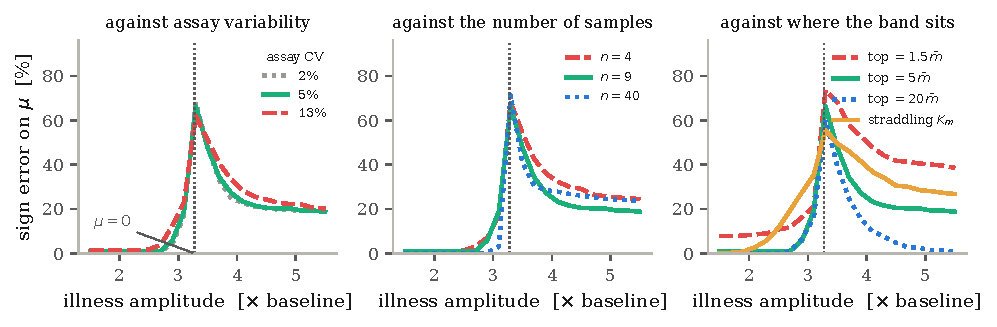
\includegraphics[width=\textwidth]{fig_D3_decision.pdf}
\caption{The probability of getting the sign of $\mu$ wrong, by simulation, as a patient of
fixed biology is swept across the decision boundary by the illness amplitude. Left of the
dotted line the error is a patient treated who did not need it; right of it, a patient left
untreated who did. Each panel varies one thing a protocol controls.}
\label{fig:D3}
\end{figure}

\begin{center}
\footnotesize
\begin{tabular}{@{}rrlrr@{}}
\toprule
\textbf{illness} & $\mu$ & \textbf{which error} & \textbf{simulated} &
\textbf{a delta method would say} \\
\midrule
$1.50\times$ & $+2006$ & treat unneeded & $0.2\%$  & $39.5\%$ \\
$2.50\times$ & $+876$  & treat unneeded & $0.2\%$  & $38.8\%$ \\
$2.98\times$ & $+339$  & treat unneeded & $6.0\%$  & $36.1\%$ \\
\addlinespace
$3.58\times$ & $-339$  & fail to treat  & $\mathbf{52.5\%}$ & $42.3\%$ \\
$4.00\times$ & $-818$  & fail to treat  & $31.8\%$ & $41.1\%$ \\
$5.50\times$ & $-2513$ & fail to treat  & $26.0\%$ & $40.4\%$ \\
\bottomrule
\end{tabular}
\end{center}

\textbf{The two errors are not the same size, and the larger one is the one that costs a
patient a decompensation.} At equal distance from the boundary --- $|\mu| = 339$ on either
side --- the simulated error is $6\%$ for treating a patient who did not need it and $53\%$
for failing to treat one who did. The asymmetry does not close with distance: at
$|\mu| = 2513$ on the unsafe side the error is still $26\%$, where at $|\mu| = 2006$ on the
safe side it is $0.2\%$. \textbf{The estimator fails towards declaring patients safe.} The
mechanism is already in this note: by Remark~\ref{rem:eiv} the abscissa noise inflates
$\hat a$ and hence $\hat\theta$, and $\hat\mu = \hat\theta - \thc$ inherits that bias
whole.

The simulated error exceeds $10\%$ for every illness amplitude from $3.10\times$ baseline
upward, which is the whole region at and beyond the decision boundary at $3.28\times$. A
protocol reporting this design's answer would be reporting a test that is nearly reliable
where it does not matter and close to a coin toss where it does.

\textbf{What excursion would fix it, and whether one exists.} Asking the same question of a
patient $30\%$ below the threshold, the simulated sign error falls from $36\%$ at a
two-fold excursion to $10\%$ at twenty-fold and then \emph{plateaus near $6\%$}: past about
forty-fold, more excursion buys nothing. The plateau is the load-bias degeneracy of
Proposition~\ref{prop:excitation}(2), which excursion does not touch. So there is no
excursion, survivable or otherwise, that delivers a $5\%$ sign error at this load record ---
and the requirement that does bite, a twenty-fold excursion for a one-in-ten error, is a
severe decompensation. Table~\ref{tab:spec} carries the whole curve.

\begin{remark}[Why this is simulated and not propagated]
\label{rem:no_delta}
A delta-method calculation, propagating the estimator's covariance to $\mu$ and reporting
$\Phi(-|\mu|/\operatorname{sd}(\hat\mu))$, is available and is wrong here, in a way that
matters. At the accessible design $\operatorname{sd}(\hat\mu)/|\mu| = 3.7$, so a Gaussian
of that width crosses zero about $39\%$ of the time. Simulating the same model instead,
$\hat\theta$ ranges over three orders of magnitude across replicates --- the design really
is that bad --- and $\hat\mu$ never changes sign.

The two disagree because $\hat\mu$ is not symmetric about $\mu$. The design's near-null
direction is very nearly the direction along which $\mu$ is monotone and of one sign, so the
sampling distribution of $\hat\mu$ is heavily skewed and does not cross zero anything like
as often as its standard deviation suggests. \textbf{That is the margin theorem of
\eqref{eq:mufibre} showing up in the estimator}, and taking the Gaussian tail at face value
would throw away the one favourable result this note has. Both numbers are reported by the
code so that the gap stays visible.
\end{remark}

\vspace{0.5em}
\hrule
\vspace{1em}

%==========================================================================
